\section{Technical Realization}
\label{sec:implementation}

In this chapter we will deal with the infrastructure and technical implementation of the public display survey platform. First off we will start with the requirements for the survey platform (section \ref{4a_requirements}). Subsequently the architecture for the platform will be our main focus (section \ref{4b_architecture}). To facilitate the training period for successors we will also take a look at the software model (section \ref{4c_modeling}) and the implementation (section \ref{4d_implementation}). For more specific information regarding maintenance or for other students extending this project, please refer to the Documentation in the Appendix.

In figure \ref{fig:4-pdsurvey-platform} a brief overview of the \textit{PDSurvey} platform and its components is given. The platform consists of three major parts: a backend for display providers (PDAdmin), a RESTful server (PDServer) and the user interface itself, being embeded on the end user devices (public displays, tablets, smartphones or other devices). Should a component not support HTML and JavaScript execution, then the required surveys can still be communicated directly with the REST API of PDServer.

\begin{figure}%[btph]
    \begin{center}
        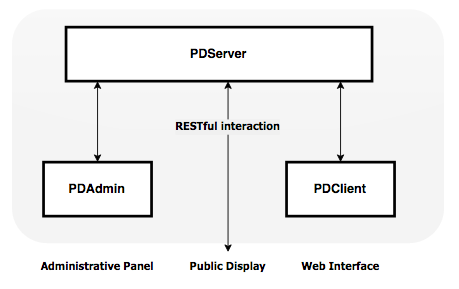
\includegraphics[width=.7\columnwidth]{img/4_implementation/4-overview}
    \end{center}
 \caption{Overview of the PDSurvey platform}
 \label{fig:4-pdsurvey-platform}
\end{figure}

 For administrative purposes we created a RESTful backend (PDBackend), 


which enables the creation, management and distribution of surveys to public displays. Attached to this backend there is the   a responsive client 

backend for administrators (built with Angular.js and Bootstrap) and a simplified version of 


\subsection{Requirements}
\label{4a_requirements}

%%% REQUIREMENTS of PROPOSAL %%%
Analyzing the problem statement and scope of the thesis, the following requirements can be derived:

\begin{enumerate}[itemsep=0pt] 
\item development of a survey tool that allows interactive public display installations to be comprehensively assessed 
\item a web-based survey platform will be implemented that can easily be used to evaluate and compare public displays through different channels 
\item different channels to support: 1) evaluation directly at
the display or 2) through a (mobile) website that allows participation also via a smartphone
or tablet.
\item configuration options for public display owners
\end{enumerate}


%%% TECHNICAL REQUIREMENTS %%%
Requirements derived from the problem statement and scope of the thesis:

\begin{enumerate}
\item JavaScript embed code, for public displays
\item supporting multiple devices: public displays, mobile (smartphone, tablet), desktop
\item responsive web design
\end{enumerate}

Additional requirements, self proposed:
\begin{enumerate}
\item scalable
\item modular / extensible
\item multilingual / internationalization (i18n)
\end{enumerate}



\clearpage

%%% Anforderungen an die Plattform %%%
\subsection{Architecture}
\label{4b_architecture}

\begin{figure}%[btph]
    \begin{center}
        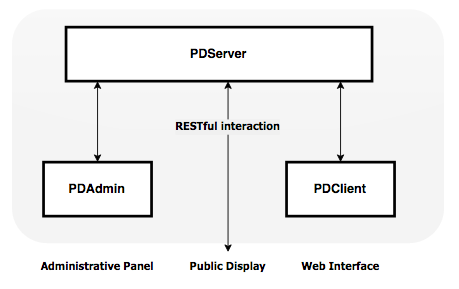
\includegraphics[width=.7\columnwidth]{img/4_implementation/4-overview}
    \end{center}
 \caption{Overview of the PDSurvey platform}
 \label{fig:4-pdsurvey-platform}
\end{figure}


The architecture for the public survey platform can be split into the following five sections:

% Overview, general requirements. Discuss all parts: 
\begin{enumerate}[itemsep=0pt] 
\item Back-end (Node.js, give reasons)
\item Front-end (Responsive)
\item API (REST)
\item Hosting
\end{enumerate}

% + state after each subsubsection why I chose which technologies and why
In the following we will first give an overview of the possible technologies and discuss why I opted for which technology.




%%  PROGRAMMING LANGUAGE  %%
\subsubsection{Programming language}

\paragraph{Categories}

\begin{enumerate}
\item Backend
\item Frontend
\item Mobile
\item Database
\end{enumerate}

% ------------------------------------- % 


\paragraph{Options}


\begin{enumerate}
\item \textbf{JavaScript}

    \begin{itemize}
        \item can be used for all platforms: front-end, back-end, public display
        \item \url{http://www.sitepoint.com/javascript-internet-things/}
        \item \textbf{Front-end}: Reasons why I chose Angular.js and not Backbone.js or Amber.js \url{https://www.airpair.com/js/javascript-framework-comparison}
        \item \textbf{Backend}: Why I chose Node.js
        \item Frameworks in Node.js: Connect, Express, Koa, ... which ones I chose why
        \item Discussion of pro/con Node.js: http://www.heise.de/developer/artikel/2x-Nein-4x-Ja-Szenarien-fuer-Node-js-2111050.html
        \item Prinzip und Verwendung von Middlewares in Node.js (wegen der Internationalisierung und Authentisierung) http://www.heise.de/developer/artikel/REST-Webservices-mit-Node-js-Teil-1-Connect-als-Fundament-1802258.html?view=print

    \end{itemize}
    
\item \textbf{Other languages}

    \begin{enumerate}
    \item PHP
    \item Python
    \item Ruby
    \item Java
    \item ASP.NET
    \end{enumerate}

\end{enumerate}
    





%%  API  %%
\subsubsection{API}

\begin{itemize}
\item REST vs SOAP
\item why I chose REST
\end{itemize}

My REST API Design, using sub-resources \url{http://code.tutsplus.com/tutorials/restful-api-design-with-nodejs-restify--cms-22637}




%%  DATABASE  %%
\subsubsection{Database}

Another fundamental aspect presented the underlying database technology, storing all of the data. A big variety of professional and open-source database management systems (DBMS) already exist on the market, but ...

Criteria for choosing the right DBMS for this project: popularity, size of community, suitability for prototyping, integration with Node.js/Angular.js

% Comparison in between ...

% My choice

Not only due to it's popularity, but also 
% - wanted to learn something new
% - popular in industry
% - MEAN stack


\paragraph{SQL: MySQL}

\begin{enumerate}
\item http://www.mysql.com/
\item "MySQL ist aus gutem Grund das Arbeitstier der Open-Source-Welt geworden: Es bietet viele der M\"oglichkeiten grosser kommerzieller Datenbanken - und ist dabei kostenlos. In seiner aktuelen Form ist MySQL performant und besitzt viele Features." \cite{hughes2012einfuhrung} (Quelle: Buch - Einf\"uhrung in Node.js, Tom Hughes-Croucher \& Mike Wilson, O'Reilly, Seite 134)
\end{enumerate}


\paragraph{SQL: PostgreSQL}

\begin{enumerate}
\item http://www.postgresql.org/
\item "Postgres (sp\"ater PostgreSQL) ist ein objektorientiertes RDBMS, das urspr\"unglich an der University of California in Berkeley entwickelt wurde. Vater des Projekts war Professor Michael Sonebraker, der es als Nachfolger seines \"alteren Ingres-Datenbank-Systems ansah. [...] Nach der Zeit in Berkeley übernahmen Open-Source-Entwickler das Projekt, ersetzten den ursprünglichen QUEL-Sprachinterpreter durch einen SQL-Sprachinterpreter und benannen das Projekt in PostgreSQL um." \cite{hughes2012einfuhrung} (Quelle: Buch - Einf\"uhrung in Node.js, Tom Hughes-Croucher \& Mike Wilson, O'Reilly, Seite 141)
\end{enumerate}


\paragraph{NoSQL: CouchDB}

\begin{enumerate}
\item http://couchdb.apache.org/
\item "CouchDB bietet einen MVCC-basierten (Multi-Version Concurrency Control) Dokumentenspeicher in einer JavaScript Umgebung. Werden Dokumente (Datens\"atze) in CouchDB hinzugef\"ugt oder aktualisiert, dann wird der gesamte Datensatz gespeichert und \"altere Versionen der Daten als obsolet markiert. Diese \"alteren Versionen des Datensazes k\"onnen immer noch in die neueste Version \"ubernommen werden, aber es wird immer eine neue Version erzeugt und f\"ur einen schnellen Lesezugriff in fortlaufenden Speicherbereichen abgelegt" \cite{hughes2012einfuhrung} (Quelle: Buch - Einf\"uhrung in Node.js, Tom Hughes-Croucher \& Mike Wilson, O'Reilly, Seite 113)
\end{enumerate}

\paragraph{NoSQL: Redis}

\begin{enumerate}
\item http://redis.io/
\item "Redis ist eine In-Memory-Datenbank mit einer Schl\"ussel/Wert-Ablage, die Ihnen sehr vertraut vorkommen sollte, wenn Sie schon \"uber Erfahrungen mit Schl\"usse/Wert-Caches wie Memcache verf\"ugen. Redis wird verwendet, wenn Performance und Skalierbarkeit wichtig sind. In vielen F\"allen entscheiden sich die Entwickler daf\"ur, es als Cache f\"ur die von einer relationealen Datenbank wie MySQL empfangenen Daten einzusetzen, auch wenn es deutlich mehr kann." \cite{hughes2012einfuhrung} (Quelle: Buch - Einf\"uhrung in Node.js, Tom Hughes-Croucher \& Mike Wilson, O'Reilly, Seite 121)
\end{enumerate}

\paragraph{NoSQL: MongoDB}

"NoSQL databases came back into the mainstream when developers needed better performance and were ok with giving up the relational aspect of RDBs (unions, joins, etc)" \url{http://psitsmike.com/2012/02/node-js-and-mongo-using-mongoose-tutorial/}

\begin{enumerate}
\item http://www.mongodb.org/
\item MongoDB is document database, storing all data in the form of JavaScript objects, PHP arrays, Python dicts or Ruby hashes. This significantly facilitates the handover from JavaScript to the database management system (DBMS).
\item "Da Mongo eine JavaScript-Umgebung mit BSON-Objektspeichern (einer Bin\"ar-Adaption von JSON) mitbringt, ist das Lesen und Schreiben von Daten aus Node heraus ausgesprochen effizient. Mongo speichert eintreffende Datens\"atze im Speicher, daher ist es in Situationen mit viel Schreibvorg\"angen eine ideale Wahl. Jede neue Version bietet verbessertes Clustering, bessere Replikation und Sharding. Da die eintreffenden Datens\"atze im Speicher abgelegt werden, ist das Einf\"ugen von Daten in Mongo nicht blockierend, womit es ideal f\"ur das Protokollieren von Operationen und Telemetriedaten ist. Mongo unterst\"utzt JavaScript-Funktionen in Abfragen. Dadurch ist es beim Lesen sehr leistungsf\"ahig, so zum Beispiel bei MapReduce-Anfragen. Mit dem dokumentenbasierten Datenspeicher von MongoDB k\"onnen Sie in Eltern-Datens\"atzen auch Kind-Datens\"atze ablegen. So kann zum Beispiel ein Blogartikel mit all seinen Kommentaren in einem einzelnen Datensatz gespeichert werden, wodurch er sich auch wieder sehr schnell auslesen l\"asst."  \cite{hughes2012einfuhrung}
\end{enumerate}

Reasons for using MongoDB
\begin{enumerate}
\item ideal for lots of write procedures
\item non-blocking write operations, ideal for Node.js and for logging data (good for our future work)
\item good read performance
\item good scalability
\item fully supports JSON syntax
\item good integration with Node.js, see Mongoose\footnote{http://mongoosejs.com/}
\end{enumerate}


Notes from the MondoDB University M101JS Class
\begin{enumerate}
\item is non-relational, ideal for JSON data
\item MongoDB is schemaless. Two documents in the same collection can have different schemas.
\item MongoDB provides a good compromise between scalability/performance and the depth of funcitonality
\item Drawback: MongoDB does not support Joins or Transactions
\end{enumerate}



%%  HOSTING  %%
\subsubsection{Hosting}

For the hosting of the platform a free and easy scalable solution was of importance. Our first choice was Heroku\footnote{https://www.heroku.com/}, due to its simplicity of setup, its native support of Node.js and the seamless integration with MongoDB\footnote{https://mongolab.com/}.

% TODO: IaaS vs PaaS: https://www.youtube.com/watch?v=Q8jZHc0NS6A
% give reasons why I chose PaaS (Platform as a Service)

    % Heroku        PaaS
    % IBM BlueMix   PaaS
    % Amawon AWS    IaaS
    % self hosting  IaaS

    %   comparison  http://smashingboxes.com/ideas/heroku-vs-amazon-web-services


Alternative were Google App Engine, IBM BlueMix, Amazon Web Services (Amazon EC2) or hosting everything on local or virtualized machines at our university. However for our scenario all of the above options had their drawbacks in comparison to Heroku. Google App Engine (as of December 2014) still had no native support for Node.js and custom runtimes had to be used to get Node.js support up and running. IBM BlueMix just got overhauled, offered full out-of-the-box Node.js support, however they only the first 30 days were free and the pricing model wasn't as attractive. Amazon Web Services offering a Infrastructure as a Service (IaaS), would have required too much administration of the server, which would have slowed down the main objective of the project, the development of the survey platform. The same goes for the last option, hosting a MEAN-stack environment on our own servers at LMU Munich. All of the above are well-known solutions in the industry, however due to simplicity and ease of use we chose Heroku.



\paragraph{Database}

http://mongoosejs.com/ + https://mongolab.com


\clearpage
\subsection{Modeling}
\label{4c_modeling}

	The model for the \textit{PDSurvey} platform is maintained with the help of the Node package Mongoose. Node.js maps the route parameters and routes all requests to the corresponding Mongoose model. Angular.js builds its model upon the REST API and maps it via dynamic two-way-binding to it's scope. Thus all changes to the model originate from Mongoose.



\subsubsection{Development Process / Modeling}

	The development process of the PDSurvey platform was inspired and influenced by the following approaches:

	\begin{itemize}
	\item working agile and user centered... TODO: look up how to best explain it.

	\item User Centered Design: (paper nr 31): ``constitutes an iterative process of system design, deployment and evaluation'' (quote from paper 31). Work iteratively, continuous deployment and evaluation.

	\item Concept of extreme programming\footnote{\url{http://www.extremeprogramming.org/rules.html} (accessed on November 14, 2014)}: First user stories were written and assessed in a small group. The next step was to transfer these stories to user models, describing in detail which functionality the stakeholders of PDSurvey are supposed to have. Later a first software architecture and software model was built, getting more specific. Dependencies between models were defined and this model was continuously refined and improved throughout the dvelopment phase. The last step of the modeling represented screen designs, getting a clear view of what the interface might later look like.

	\item Used the extreme programming\footnote{\url{http://www.extremeprogramming.org/rules.html} (accessed on November 13, 2014)} approach: user stories, release planning, release schedule, small releases, iterating


	\item criteria for good user stories: http://tigertechtalk.wordpress.com/2012/10/17/wie-schreibe-ich-eine-gute-user-story-und-was-ist-das-uberhaupt/
	\end{itemize}








\subsubsection{User roles}

As of now only two roles are implemented, the admin-role and the guest-role.

% FEEDBACK VON FLORIAN: nein, nicht zu komplex machen. Es sollte sogar reichen, nur zwischen Admin & Operator (= Application Provider) zu unterscheiden, da der end user (das Public Display) ja sowieso nur auf die öffentlichen REST API Zugriff hat. (2014-11-14)


In the long term it would be desirable to have the following user roles: Admin, Operator, Evaluator, DisplayApplication.






\subsubsection{Software model}

In total there are the following classes.

\begin{enumerate}
\item list all classes
\item 1 UML diagram is enough, according to Florian
\end{enumerate}


\subsubsection{Dependencies}

Of special interest are the following four models: Survey, Display, Campaign and Responses.

\paragraph{Surveys:} Surveys resembles the foundation of PDSurvey, with the aim of reuse and standardization. A survey consists of multiple sections, being built of of multiple questions. Each question is of a corresponding question type and every survey belongs to a category. This allows the filtering for relevant surveys. To be able to create private surveys, not being shared across the entire platform, every survey is assigned to an individual user.

\paragraph{Displays:} In the display collection all displays connected to the PDSurvey platform are contained. To allow for an evaluation across multiple display models and based on the context of the displays, the display model and a static and/or dynamic context is assigned to every display.

\paragraph{Campaigns:} Campaigns resemble the most integral part, since they glue all of the pieces together and allow the distribution of surveys to public display networks. A campaign consists of displays and surveys and creates the mapping of the questionnaires to public displays. Additionally to each of those mapping an individual context can be assigned, enabling the later comparison of results in between the public displays.

\paragraph{Responses:} All responses made to each survey are logged in the Response collection. The queries are carried out individually per user, per display and per campaign. This model will be the base for further extensions, amongst others the automatic evaluation of the survey responses and the comparison inbetween an entire display network, to be able to find out which properties of a display might be related to certain effects.

\paragraph{Context:} One of the benefits of creating such a survey platform is being able to collect and evaluate large amounts of data, without having to pay more people for conducting and evaluating the survey. The idea would be to collect a large number of responses from a variety of displays in various settings, and assigning a specific context to every display connected to PDSurvey. Once enough data is collected, having the ability to evaluate and compare the displays between each other. Interesting questions for analysis would be, which role the context plays on how the users behave, when running identical software settings on the displays, but only varying the context (position, size of display, surrounding environment of the display, positioning it outdoors or indoors, influence of the weather, type of building it is positioned in).


\begin{figure}%[btph]
    \begin{center}
        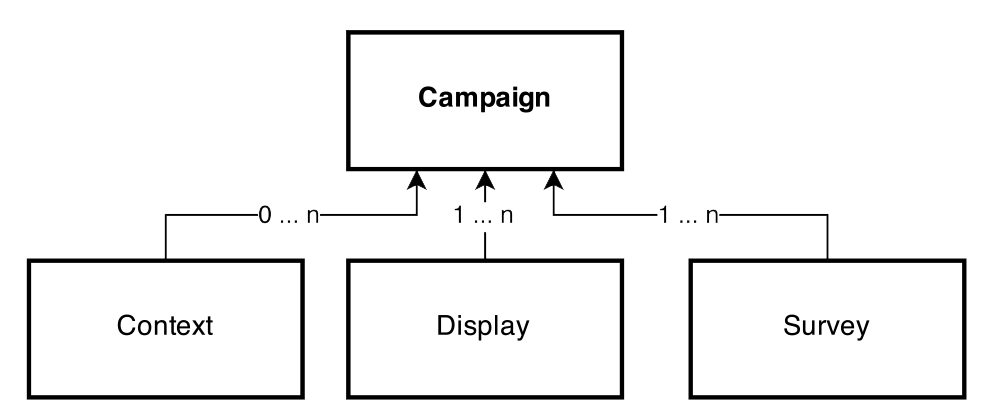
\includegraphics[width=.8\columnwidth]{img/4_implementation/4-dependency-campaign}
    \end{center}
 % \begin{center}\LARGE [BILD]\end{center}
 \caption{Campaign model dependencies}
 \label{fig:4-dependency-campaign}
\end{figure}


++ neue Namensgebung, um in der domain specific language zu bleiben --> application provider / display provider / space provider (anstatt Operator). Wir werden aber nur mit dem Application Provider (anstatt Operator) im System arbeiten





\subsubsection{REST interface}

Defining the REST API. 

% TODO: Explain why I chose which level of separation / detail.

Notes from before I started writing: 
\begin{enumerate}
\item Think about using a Extreme Programming approach http://www.extremeprogramming.org/rules.html
\end{enumerate}

\clearpage
\subsection{Implementation}
\label{4d_implementation}


Briefly describe how I approached the implementation.

\begin{enumerate}
\item Challenges
\item Problems
\item ...
\end{enumerate}


\subsubsection{Package Manager}

\begin{enumerate}
\item NPM and Bower (instead of Browserify) + state reasons
\item State reasons, why I did / didn't check in the code for npm / bower components: \url{http://addyosmani.com/blog/checking-in-front-end-dependencies/}

    \begin{itemize}
    \item "prevent bad dependencies from breaking their app"
    \item "the longevity of package managers and their tooling"
    \item to be independent of other services and thus to garantee a longer life for the tool
    \end{itemize}
\end{enumerate}



\subsubsection{Frontend Framework}

give an overview of current Frontend Frameworks and briefly state which one I used why. A good comparision can be found here \url{http://www.sitepoint.com/5-most-popular-frontend-frameworks-compared/}

\begin{enumerate}
\item Bootstrap
\item Foundation by Zurb
\item ...
\end{enumerate}



\subsubsection{Deployment}

Practical deployment, best practices, how I proceded, and why

\begin{enumerate}
\item GitHub Repo
\item Deployment to Heroku
\end{enumerate}